\documentclass[../main.tex]{subfiles}
\ifSubfilesClassLoaded{\setcounter{chapter}{11}}{}
\begin{document}

\chapter{Metrik Klasifikasi Lanjut dan ROC-AUC Opsional}

\begin{subcpmk}
  \item \textbf{Sub-CPMK-P9:} Presisi, recall, F1; ROC-AUC untuk kasus biner; diskusi ketidakseimbangan kelas (RPS Mg.\ 11).
\end{subcpmk}

\SesiRPS{11}{P9}{$\sim$170 menit}{CPMK-P4}

\noindent Akurasi saja sering gagal menggambarkan biaya kesalahan yang tidak simetris. Presisi dan recall memisahkan dua jenis risiko: alarm palsu versus kejadian yang terlewat---sangat relevan untuk deteksi fraud, diagnosis, atau moderasi konten.

\section{Kemampuan akhir sesi}

Menghitung dan menjelaskan presisi, recall, dan F1; membaca kurva ROC dan AUC untuk kasus biner; mendiskusikan dampak ketidakseimbangan kelas pada pemilihan metrik dan threshold.

Pada data tidak seimbang, pertimbangkan \texttt{class\_weight} atau sampling dengan hati-hati; dokumentasikan trade-off karena teknik sampling dapat mengubah distribusi target secara artifisial.

\section{Teori}

\begin{konsep}
Presisi menjawab ``dari yang diprediksi positif, berapa yang benar''; recall ``dari semua positif sejati, berapa yang tertangkap''. F1 adalah harmonik keduanya. ROC-AUC bermakna kuat pada klasifikasi biner dengan skor probabilitas.
\end{konsep}

ROC mengintegrasikan trade-off TPR/FPR pada berbagai threshold; AUC mendekati 0.5 menandakan skor hampir acak. Untuk multiclass, laporan per kelas dan rata-rata makro/mikro memberi gambaran yang lebih lengkap daripada satu angka.

\begin{figure}[htbp]
\centering
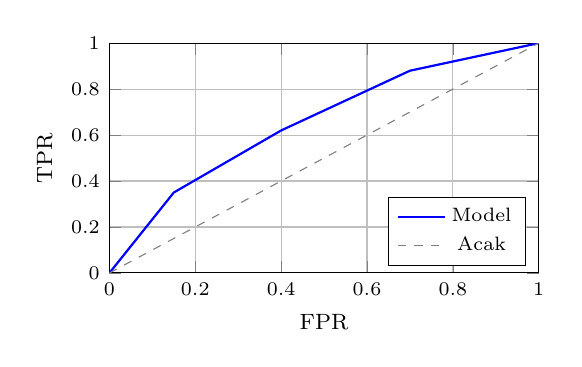
\begin{tikzpicture}
\begin{axis}[
  width=0.58\textwidth,
  height=4.5cm,
  xmin=0, xmax=1,
  ymin=0, ymax=1,
  xlabel={\footnotesize FPR},
  ylabel={\footnotesize TPR},
  grid=major,
  tick label style={font=\scriptsize},
  legend style={font=\scriptsize, at={(0.97,0.03)}, anchor=south east}
]
\addplot[thick, blue] coordinates {(0,0) (0.15,0.35) (0.4,0.62) (0.7,0.88) (1,1)};
\addplot[dashed, gray] coordinates {(0,0) (1,1)};
\legend{Model, Acak}
\end{axis}
\end{tikzpicture}
\caption{Ilustrasi kurva ROC untuk klasifikasi biner: diagonal putus-putus = baseline acak; kurva di atasnya menandakan pemisahan kelas yang lebih baik (AUC lebih besar).}
\end{figure}


\begin{table}[htbp]
\centering
\caption{Kapan mementingkan presisi vs recall (contoh domain).}
\label{tab:precision-recall-domain}
\begin{tabular}{@{}>{\raggedright\arraybackslash}p{3.6cm}>{\raggedright\arraybackslash}p{9.1cm}@{}}
\toprule
\textbf{Skenario} & \textbf{Prioritas metrik} \\
\midrule
Deteksi penyakit serius & Recall tinggi (minimal FN). \\
Kampanye pemasaran & Presisi tinggi (minimal FP). \\
\bottomrule
\end{tabular}
\end{table}

\section{Contoh kode}

\noindent\textbf{Mengapa blok ini?} Dataset kanker payudara adalah klasifikasi biner; \path{classification_report} merangkum precision/recall/F1; \path{RocCurveDisplay.from_estimator} memplot TPR vs FPR dari \path{decision_function} LogReg; \path{f1_score(..., average="macro")} rata-rata F1 antar kelas tanpa bobot frekuensi.

\begin{lstlisting}[caption=ROC curve + classification report (biner)]
from sklearn.metrics import classification_report, RocCurveDisplay, f1_score
from sklearn.linear_model import LogisticRegression
from sklearn.datasets import load_breast_cancer
from sklearn.model_selection import train_test_split

X, y = load_breast_cancer(return_X_y=True)
X_train, X_test, y_train, y_test = train_test_split(
    X, y, test_size=0.25, random_state=42, stratify=y
)
clf = LogisticRegression(max_iter=5000)  # data berskala besar butuh iterasi solver lebih banyak
clf.fit(X_train, y_train)
y_pred = clf.predict(X_test)  # threshold default 0.5 pada skor linear
print(classification_report(y_test, y_pred))  # per kelas + weighted avg
print("F1 macro", f1_score(y_test, y_pred, average="macro"))
RocCurveDisplay.from_estimator(clf, X_test, y_test)  # kurva ROC memakai y_true dan skor kontinu dari clf
\end{lstlisting}

\noindent\textbf{Mengapa blok ini?} \texttt{precision\_recall\_fscore\_support} mengembalikan array per kelas Iris; \texttt{zip} menggabungkan metrik dengan \texttt{support} (jumlah sampel uji per kelas).

\begin{lstlisting}[caption=Precision/Recall per kelas (multiclass)]
from sklearn.metrics import precision_recall_fscore_support
from sklearn.datasets import load_iris
from sklearn.model_selection import train_test_split
from sklearn.linear_model import LogisticRegression

X, y = load_iris(return_X_y=True)
X_train, X_test, y_train, y_test = train_test_split(
    X, y, test_size=0.25, random_state=42, stratify=y
)
m = LogisticRegression(max_iter=200).fit(X_train, y_train)  # pola method chaining: construct lalu fit
yp = m.predict(X_test)
p, r, f, sup = precision_recall_fscore_support(y_test, yp)  # empat array paralel per kelas
print(list(zip(p, r, f, sup)))  # pasangkan metrik per indeks kelas
\end{lstlisting}

\begin{contoh}
Di sel Markdown: jelaskan skenario di mana \textbf{recall} lebih penting daripada \textbf{precision} (mis.\ deteksi fraud) dan sebaliknya (mis.\ kampanye email).
\end{contoh}

\section{Referensi}

\begin{itemize}[leftmargin=*]
  \item sklearn model evaluation. \url{https://scikit-learn.org/stable/model_evaluation.html}
\end{itemize}

\begin{asesmen}
\textbf{Rubrik sesi:} metrik selaras distribusi kelas; narasi untuk pemangku kepentingan non-teknis satu paragraf.
\end{asesmen}

\begin{rangkuman}
Minggu 11 mendalami evaluasi di luar akurasi semata.

\textbf{Kata kunci:} precision, recall, F1, ROC-AUC
\end{rangkuman}

\end{document}
